\documentclass[
reprint,amsmath,amssymb,aps]{revtex4-2}

\usepackage{graphicx}
\usepackage{dcolumn}
\usepackage{bm}
\usepackage{float}
\usepackage{tabularx}
\usepackage{multirow}
\usepackage{braket}
\usepackage{amsmath}


\begin{document}

\preprint{APS/123-QED}

\title{Spin dynamics and magnetic bistability in single Dy adatoms on graphene/Ir(111)
studied by SP-STM}

\author{A. Curcella}
\affiliation{Institute of Physics, Ecole Polytechnique Fédérale de Lausanne, CH-1015 Lausanne, Switzerland}

\author{D. Sblendorio}
\affiliation{Institute of Physics, Ecole Polytechnique Fédérale de Lausanne, CH-1015 Lausanne, Switzerland}

\author{S. Rusponi}
\affiliation{Institute of Physics, Ecole Polytechnique Fédérale de Lausanne, CH-1015 Lausanne, Switzerland}

\author{M. Pivetta}
\affiliation{Institute of Physics, Ecole Polytechnique Fédérale de Lausanne, CH-1015 Lausanne, Switzerland}

\author{F. Patthey}
\affiliation{Institute of Physics, Ecole Polytechnique Fédérale de Lausanne, CH-1015 Lausanne, Switzerland}

\author{H. Brune}
\affiliation{Institute of Physics, Ecole Polytechnique Fédérale de Lausanne, CH-1015 Lausanne, Switzerland}
 

\begin{abstract}
%The magnetic stability in single Dy adatoms on graphene/Ir(111) is investigated by means of spin-polarized scanning tunneling microscopy at liquid He temperature. Telegraph-noise traces demonstrate the bistability of the Dy magnetization, and exhibit long relaxation times of several minutes, consistent with previous XMCD measurements \citep{baltic2016}.
%The asymmetric occupancy of the magnetic states as a function of tunnel voltage is evidence for a spin-torque exerted by tunneling electrons on the single-atom magnet \citep{Khajetoorians2013,delgado2010}.
%Based on existing theoretical works, we implement a model that quantitatively reproduces the asymmetry in the occupancy of the magnetic states and their average lifetimes, the temperature dependence of the magnetization reversal, and the value of the magnetoresistive contribution in the STM current. 
\end{abstract}

\maketitle


%Manipulation of the magnetic states of nano-objects and in surface adsorbed single adatoms offer novel avenues for exploring the fundamental physics that determine their behavior. Understanding this behavior is essential for the development of future spintronic devices and the realization of ultra-high-density magnetic memory [citations...]. The injection of a spin-polarized current can efficiently reorient the magnetization of a nanomagnet \citep{Khajetoorians2013,krause_joule_2011,loth2010}, enabling the possibility of reading and writing of the magnetic states.
%Dysprosium atoms adsorbed on a single graphene layer grown on Ir(111) were identified as stable single-atom magnets \citep{baltic2016}. Previous scanning tunneling microscopy (STM) studies revealed these atoms self assemble into a highly-ordered superlattice after annealing at 40~K \citep{baltic2016,pivetta2018}. Obtaining uniformly dispersed bistable magnetic nanostructures on a decoupling atomic layer is a paramount achievement for the development of ultra-high magnetic memory densities [citations]. Previous x-ray magnetic circular dichroism (XMCD) measurements revealed that Dy adatoms on graphene/Ir(111) possess a \textit{4f$^{\:10}$} occupation, a \textit{J} = 8 total angular momentum identical to Dy in the gas phase, and a \textit{J$_z$} = $\pm$7 out-of-plane magnetic ground state \citep{baltic2016,baltic2018}. The measured spin lifetimes are of the order of 1000~s at 2.5~K.
%However, the lifetimes obtained by XMCD are limited by the interaction of the adatoms with photon-induced secondary electrons. The extrapolation of the intrinsic magnetization lifetime at zero photon flux represents a lower bound estimate.

Coherent spin manipulation and reading/writing the state of stable single-atom magnets represent two of the milestones of modern spintronics research \cite{Natterer2017,yang2019}. These achievements pave the way towards the realization of coherent spintronic devices and ultra-high density memories based on atomic-scale objects. The former application requires adatoms with a long coherence time and efficient spin manipulation \cite{baumannElectronParamagneticResonance2015,yang2019}, while the latter relies on adatoms showing magnetic remanence \cite{baltic2018,donatiMagneticRemanenceSingle2016,Natterer2018} or, as well, bistability in the orbital population \cite{kiralyOrbitallyDerivedSingleatom2018}. The interaction with the environment and the probing method greatly influence these properties in magnetic adatoms \cite{malavolti_MinimallyInvasiveSpin_2020,verlhacAtomicscaleSpinSensing2019a}. A comprehensive record of such interactions can show new ways of tailoring the properties of single-atom magnets, making them suitable for a wide range of applications \cite{kiraly_AtomicBoltzmannMachine_2021,khajetooriansRealizingAllSpinBased2011}.

In the present work, we demonstrate how intra-atomic exchange interaction affects the spin dynamics of isolated Dy atoms adsorbed on a single graphene (gr) layer grown on Ir(111). Dy/gr/Ir(111) is one of the few examples of single atom magnets \cite{Natterer2018,kiralyOrbitallyDerivedSingleatom2018} with spin lifetimes of the order of 1000~s at 2.5~K \cite{baltic2016}. Despite lacking the thermal stability reported for Ho/MgO/Ag(100), this system has other unique properties. Firstly, Dy adatoms self-assemble on the Moiré pattern of gr/Ir(111) after annealing at 40 K \cite{pivettaDirectCaptureElectrostatic2018}. Secondly, it shows an unrivaled magneto-resistive contrast in spin-polarized scanning tunneling microscopy (SP-STM) measurements \cite{pivettaMeasuringIntraAtomicExchange2020}. One can thus obtain an ordered bidimensional array of atomic bits, characterized by a low bit error rate.
However, the spin dynamics governing the bistability of the magnetization in the Dy adatoms still lacks a quantitative  description.
In the following, we present the results of SP-STM  measurements conducted  on  well-isolated  Dy  adatoms on gr/Ir(111). We implement a model which accounts for the  recently  observed  intra-atomic  interaction  between internal \textit{4f} and  external \textit{5d6s} polarized  shells  \cite{pivettaMeasuringIntraAtomicExchange2020}, offering new insights in the spin dynamics  of  rare-earth  based  single-adatom  magnets.

The Dy adatoms adsorb onto the 6-fold symmetrical ($C_{6v}$) graphene hollow site \cite{baltic2018}. The crystal field lifts the degeneracy of the magnetic states and gives rise to a strong out-of-plane easy-axis anisotropy.
If the intra-atomic exchange is neglected (\textit{i.e.} the external shells are not polarized), the magnetic states $\ket{M}$ are defined solely by the spin of the \textit{4f} shell $\ket{M}=\ket{j_{4f}}$ (Fig.~\ref{fig:intra}a). The zero-field level scheme of Dy system, in this case, is depicted in Fig.~\ref{fig:intra}b. The term $B_6^6$ in the crystal field Hamiltonian term (see Supplemental) mixes the states with $\Delta j_{4f}=6n$, with $n\in \mathbb{Z}$. The states $\ket{j_{4f}}=\ket{\pm 6}$ are therefore mixed, with a splitting of $\omega=1.3 \times 10^{-2}$ meV. The mixing of these states permits the only efficient channel for magnetization reversal, via quantum tunneling of magnetization (QTM), at energies $E<20$ meV \citep{baltic2016}. The inclusion of the intra-atomic exchange term in the Hamiltonian (\textit{i.e.} the external shells are polarized), produces a modified level scheme. In addition to the spin of the \textit{4f} shell, the new basis includes the spin of the valence \textit{5d6s} shell $\ket{M}=\ket{m_i}=\ket{j_{4f},s_{5d},s_{6s}}$ (Fig.~\ref{fig:intra}d). The intra-atomic exchange couples the \textit{4f} and the \textit{5d6s} shells ferromagnetically (Fig.~\ref{fig:intra}f) \cite{pivettaMeasuringIntraAtomicExchange2020}. 
In this new basis, the $B_6^6$ term of the crystal field mixes the states with $\Delta M_{tot}=\Delta j_{4f} + \Delta s_{5d} + \Delta s_{6s}=6n$, $n\in \mathbb{N}$. This results in the mixing and splitting of the states $\ket{M}=\ket{m_{\pm 5}}$ and $\ket{M}=\ket{m_{\pm 8}}$ (Fig.~\ref{fig:intra}e), which have $\Delta M_{tot}\sim 10+1+1 = 12$ and $\Delta M_{tot}\sim 16 +1+1=18$, respectively. With respect to the former case, two magnetization reversal pathways via QTM exist, the first between $\ket{m_{5}}$ and $\ket{m_{-5}}$, and the second between $\ket{m_{8}}$ and $\ket{m_{-8}}$. Thus, the pathways for the magnetization reversal are unique to the choice of the basis. 

\begin{figure*}[ht!]
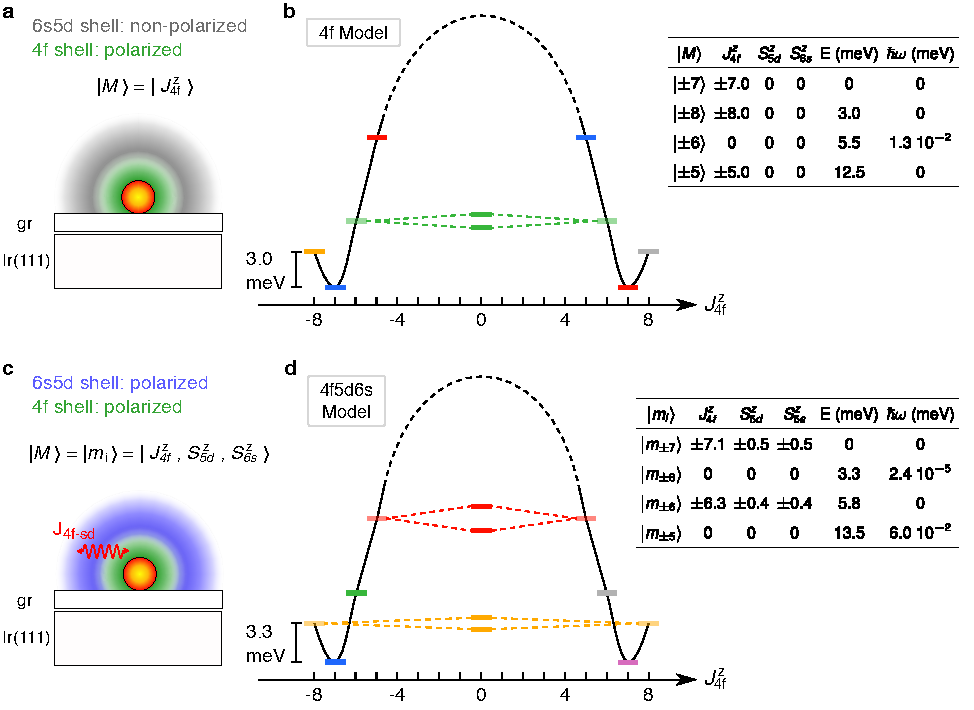
\includegraphics[width=0.98\textwidth]{Fig1_new.pdf}
\caption{Comparison of the polarized and non-polarized models. (\textbf{a}) Choice of the basis and sketch of the system for the model that considered an unpolarized \textit{5d6s} shell. (\textbf{b}) Corresponding level scheme for the description in (\textbf{a}). States with the same color are mixed by the crystal field. The green dotted line represent the mixing and energy splitting (exaggerated for clarity) of $\ket{\pm6}$ states. Higher energy states are not relevant in the present work.  (\textbf{c}) Values of the out-of-plane magnetic moment projection for internal ($j_{4f}$) and external ($s_{5d}$, $s_{6s}$)  electronic shells, energy ($E$) and energy splitting for the states $\ket{M}$ depicted in (\textbf{b}). (\textbf{d}) Same as in (\textbf{a}) for the model considering a polarized external shell. $J_{4f-sd}$ represents the intra-atomic exchange coupling between \textit{4f} and \textit{6s5d} shells. (\textbf{e-f}) Same as in (\textbf{b}) and (\textbf{c}) for the polarized model.
\label{fig:intra} }
\end{figure*}

We employ an anti-ferromagnetic MnNi tip to measure the magnetization state of an isolated Dy adatom via the magnetoresistive effect \cite{wiesendanger_ObservationVacuumTunneling_1990,Khajetoorians2013,paul_ControlMillisecondSpin_2017,Natterer2017,Natterer2018}. The fixed spin-polarization of the tip enables the measurement of the lifetimes of the ground-states $\ket{m_{\pm7}}$, the spin-lifetimes of the excited states being too short to be detected within the bandwidth of available current-sensing electronics. Fig.~\ref{fig:no_tip_tip_telegraph}b shows an example of a telegraph signal noise (TSN) trace at positive tip-sample voltage bias $V_b$ in which the tunneling current switches between a high conductance (HC) and low conductance (LC) state, corresponding to a parallel and antiparallel alignment between the majority spin-polarization at the Fermi level of the tip and the magnetization of the adatom, respectively \cite{delgado2010,paul_ControlMillisecondSpin_2017}. From a TSN trace we extract two quantities: the occupancy, defined as the fraction of time that the magnetization adatom is in the high conductance (HC) or low conductance (LC) state, and the characteristic lifetime $\tau ^*=(\tau_{HC}  \cdot \tau_{LC})/( \tau_{HC} + \tau_{LC})$, defined by the average HC and LC state lifetimes, $ \tau_{HC}$ and  $\tau_{LC}$ \cite{Khajetoorians2013}. 

We now describe the mechanisms by which the magnetization is driven out of the ground states $\ket{M}=\ket{\pm7}$ and into the higher energy states, in which QTM can occur. The intrinsic lifetime of the Dy system is limited by substrate electron and phonon scattering. In addition to these mechanisms, the measured lifetime is determined by further electron scattering channels and any stray magnetic field due to the presence of the STM tip (Fig.~\ref{fig:no_tip_tip_telegraph}a). We implement additional terms in the model Hamiltonian to account for these effects. 

\begin{figure*}[ht!]
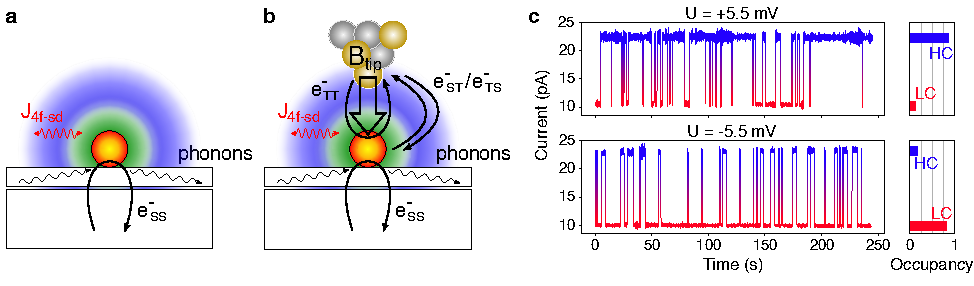
\includegraphics[width=0.98\textwidth]{Fig2_new.pdf}
\caption{STM schematic and TSN trace. (\textbf{a}) Simplified sketch of the relevant processes considered in the model that influence the measured quantities during tunneling conditions. (\textbf{b}) Sample TSN trace showing a clear asymmetry in occupancy (right graph) between high conductance and and low conductance states ($V_{b} = +5.5$ mV, $T = 6.5$ K). The elastic current $I_{o}$ is the average current measured in each trace and the magnetoresistive component $\pm I_{MR}$ is the absolute difference between $I_{o}$ and $I_{HC}$ or $I_{LC}$, respectively.
\label{fig:no_tip_tip_telegraph} }
\end{figure*}

To described the coupling between adatom and electrodes (\textit{i.e.} the tip and the substrate), we use a Kondo-type Hamiltonian consistent with previous models \cite{anderson1966,schrieffer1966,appelbaum1967,delgado2010,loth2010,Ternes2015}. Within the context of this model, scattering with the Dy adatom is defined by the inital and final electrode: substrate-substrate scattering ($e^{-}_{SS}$), tip-tip scattering ($e^{-}_{TT}$), and tip-substrate/substrate-tip scattering ($e^{-}_{TS}$/$e^{-}_{ST}$). In the case of substrate-substrate scattering, the creation or annihilation of an electron hole pair in the substrate induces a spin transition ($\Delta m=\pm 1$) in the external \textit{5d6s} shell. Consequently, the magnetic moment of the $4f$ shell flips due to the intra-atomic exchange coupling between the shells \cite{pivettaMeasuringIntraAtomicExchange2020}. We consider a non-polarized substrate, implying substrate-substrate scattering results in symmetric ($\Delta m=\pm 1$) transitions and therefore promotes equal occupancy between HC and LC states. In the case of tip-tip scattering, the creation or annihilation of an electron hole pair in the tip induces a spin transition ($\Delta m=\pm 1$) in the external \textit{5d6s} shell. The spin-polarized MnNi tip is characterized by spin-up $\rho_{T\uparrow}$ and spin-down $\rho_{T\downarrow}$ populations at the Fermi level. The asymmetry in the population implies a higher probability of spin-increasing ($\Delta m=+1$) or spin-decreasing ($\Delta m=-1$) transitions in the Dy adatom. Note that neither $e^{-}_{SS}$ nor $e^{-}_{TT}$ electrons contribute to the tunneling current, but they do affect the spin dynamics of the system. Finally, the electrons that participate in tip-substrate/substrate-tip scattering define the tunneling current. The tunneling current is composed of three contributions: elastic $I_0$, elastic magnetoresistive $I_{MR}$, and inelastic $I_{in}$. The inelastic component is several orders of magnitude lower than the elastic one. Thus, the current of the HC state and LC state can be approximated as $I_0+I_{MR}$ and $I_0-I_{MR}$, as shown in Fig.~\ref{fig:no_tip_tip_telegraph}. The transition rates associated with substrate-substrate ($e^{-}_{SS}$), tip-tip ($e^{-}_{TT}$), tip-substrate ($e^{-}_{TS}$) and substrate-tip ($e^{-}_{ST}$) can be expressed as:

\begin{equation}
    W_{MM^{\prime}}^{\eta \eta^{\prime}}=\dfrac{2\pi}{\hbar} \zeta^2 \varsigma_{\eta} \varsigma_{\eta^{\prime}} \mathcal{F}^{\eta\eta^{\prime}}(\Delta E_{M,M^{\prime}}+V_{\eta \eta^{\prime}} )  w_{MM^{\prime}}^{\eta \eta^{\prime}},
    \label{eq:elec_rates}
\end{equation}

where $\eta,\eta^{\prime}=T,S$. $w_{MM^{\prime}}^{\eta \eta^{\prime}} $ are the tunneling matrix elements squared, $\varsigma$ is the coupling between the adatom and each electrode $\eta$ and $\eta^{\prime}$. $\mathcal{F}^{\eta\eta^{\prime}}$ accounts for the state occupation for a given level splitting $\Delta E_{M,M^{\prime}}$ and tunnel bias $V_{TS/ST}$. For $\eta,\eta^{\prime}=S$ or $\eta,\eta^{\prime}=T$, $W$ describes electrons originating and ending in the same electrode ($e^{-}_{SS}$, $e^{-}_{TT}$). For $\eta = S,\eta^{\prime}=T$ or $\eta = T,\eta^{\prime}=S$, $W$ accounts for the scattering from the tunneling electrons ($e^{-}_{TS}$, $e^{-}_{ST}$). $\zeta$ represents the ratio between inelastic and elastic tunneling matrix elements, which we assume to be independent of $V_b$ and tip-sample distance \cite{fern2009,paul_ControlMillisecondSpin_2017,lorenteEfficientSpinTransitions2009,nussinovNoiseSpectroscopySingle2003}. For all the model curves presented, we find a value of $\zeta$ = 0.3 gives a good agreement between the magnitude of the experimental and simulated magnetoresistive current $I_{MR}$ \cite{delgadoSpinTransferTorqueSingle2010,delgado2010}.
$\varsigma_T$ is related to $\varsigma_S$ through the value of the elastic current $I_0$ (see Supplemental). The coupling with the substrate $\varsigma_S$ is an additional free parameter within the model. We consider it independent of the tunneling conditions and therefore constant. A value of $\varsigma_S$ = 0.065 is not only in agreement with the experimental data presented here, but also in excellent agreement with the extrapolated zero-photon flux XMCD lifetime of 971±71 seconds at 10 mT and 2.5 K \citep{baltic2016}. We find a value of 962 seconds in the absence of the aforementioned tip scattering processes or tip field $B_{tip}$. 

To account for phonon scattering in the substrate, we implement a two-dimensional phonon bath that can excite and relax the magnetic states of the Dy adatom \cite{cervetti2016,politi_tunneling_1995}. Phonons can be interpreted as a perturbation of the crystal field; acting only the external $4f$-shell due to its non-vanishing orbital component. We allow transitions with $\Delta m = \pm 1$ and $\Delta m = \pm 2$ \citep{cervetti2016}. The transition rates between the states $\ket{M}$ and $\ket{M^{\prime}}$ can be expressed as \cite{politi_tunneling_1995, cervetti2016,Leuenberger2000}:

\begin{equation}
    \label{eq:phonon_rates}
    W_{MM^{\prime}}^{ph}=\dfrac{\nu_{ph}}{\rho_{gr} \hbar^3 c^4} \mathcal{P} \left( E_{MM^{\prime}}, T \right) w^{ph}_{MM^{\prime}}
\end{equation}

where $\nu_{ph}$ is proportional to the phonon-spin coupling cross section and is equal to $6 \times 10^{-4}$, $c_{gr}$ is the speed of sound in graphene, $\rho_{gr}$ is the 2D graphene mass density. $\mathcal{P}\left( E_{MM^{\prime}}, T \right)$ depends on the Bose-Einstein distribution at the sample temperature $T$ and the energy difference $E_{MM^{\prime}}$ between states $\ket{M}$ and $\ket{M^{\prime}}$. $w^{ph}_{MM^{\prime}}$ are the phonon matrix elements, acting on the $4f$ shell (see Supplemental).

\begin{figure*}[t!]
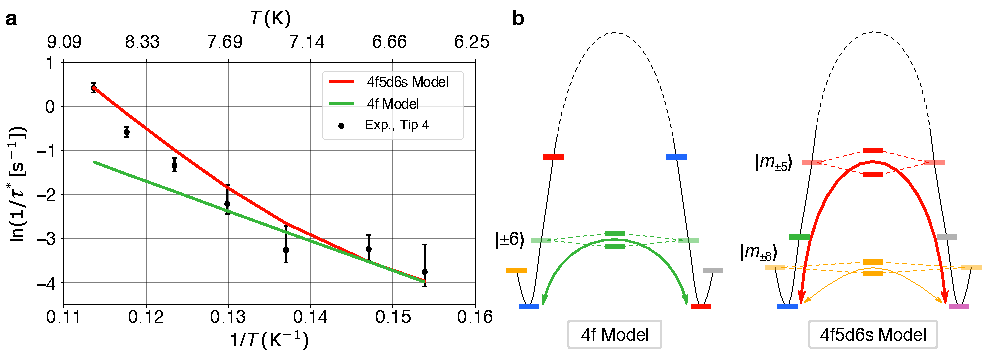
\includegraphics[width=0.99\textwidth]{Fig3_new.pdf}
\caption{Variable Temperature Measurements. (\textbf{a}) Arrhenius plot comparing the polarized (red) and non-polarized (green) models with the experimental observations (black). The average measured ratio in (\textbf{a}) and (\textbf{b}) $I_{MR}/I_{o}$ = 0.08±0.01 while the model predicted value is $I_{MR}/I_{o}$ = 0.1. Error bars correspond to 95$\%$ confidence intervals calculated using the Agresti-Coull method for binomial distributions \citep{agresti1998}. (\textbf{b}) Level scheme of the two models. The slope of the Arrhenius is determined by the height of the anisotropy barrier, and therefore manifest the differences in the reversal pathways between each model. 
\label{fig:temp} }
\end{figure*}

A Zeeman term in the Hamiltonian describes the influence of a stray magnetic field produced by the STM tip. The tip field shifts the magnetic states sitting on the opposite sides of the anisotropy barrier, resulting in an energetically preferred ground-state. This manifests experimentally as an asymmetric occupancy of $\ket{m_7}$ and $\ket{m_{-7}}$ states. Higher magnetic fields stabilize the preferred ground-state and increase the characteristic lifetime. SP-STM tips can induce both dipolar and exchange-like magnetic interactions between the tip and single adatoms at tunneling distances. Field strengths span from the mT range to as high as 10 T \cite{yang2019}. The exchange-like component of the field can have a non-trivial dependence on the tip-adatom distance and can change due to atomic-scale modifications of the tip apex \cite{hauptmannQuantifyingExchangeForces2020,tao_SwitchingSingleSpin_2009,lazoFirstprinciplesStudyMagnetic2011,lazoRoleTipSize2008}.  

Taking these mechanisms into account, we reproduce the experimental occupancy and characteristic lifetimes measured from TSN traces similar to Fig. \ref{fig:no_tip_tip_telegraph}b, as a function of bias $V_{b}$, temperature $T$, and average current $I_{o}$. The transition rates defined by Eqs.~\ref{eq:phonon_rates} and~\ref{eq:elec_rates} are used within a master equation to obtain values for $\tau^*$ and state occupancy for a certain set of tunneling conditions \cite{delgado2010,Khajetoorians2013,loth2010,cervetti2016}. We emphasize conditions where the non-polarized model fails to reproduce the experimental observations, motivating the need to include the polarized shell in order to correctly describe the relevant spin dynamics.

In Fig.~\ref{fig:temp}, we show an Arrhenius plot measured on a Dy adatom for temperatures between 6.5 K and 8.8 K. The lifetimes $\tau^*$ decrease exponentially with increasing temperature. The slope of the curve in the Arrhenius plot is related to the energy barrier of the transition enabling the magnetization reversal in the Dy adatom. In the same figure, we show the curves determined by each model described in Fig.~\ref{fig:intra}: the model which describes the intra-atomic exchange between the internal \textit{4f} shell and the polarized \textit{5d6s} shell (\textit{4f5d6s} model) and the model that considers an unpolarized external shell (\textit{4f} model). The parameters of each model have been optimized independently in order to obtain the best agreement. Most notably, the \textit{4f} model fails to reproduce the lifetimes at high temperature ($T\sim 8.8$ K). The active pathway for magnetization reversal between $\ket{6}$ and $\ket{-6}$ (see Fig.~\ref{fig:temp}b) lies at 5.5 meV, which corresponds to the slope obtained for the $4f$ model points in Fig.~\ref{fig:temp}a. Conversely, the \textit{4f5d6s} model slope increases as the temperature increases; congruent with the experimental trend. In this case the slope of the Arrhenius corresponds to a convolution of both reversal pathways. An increasing slope corresponds to substrate electrons inducing progressively more excitations towards the $\ket{-5}$ and $\ket{5}$ states due to thermal broadening. This stresses the importance of including the intra-atomic exchange in the model spin dynamics of Dy adatoms on gr/Ir(111).

\begin{figure}[h!]
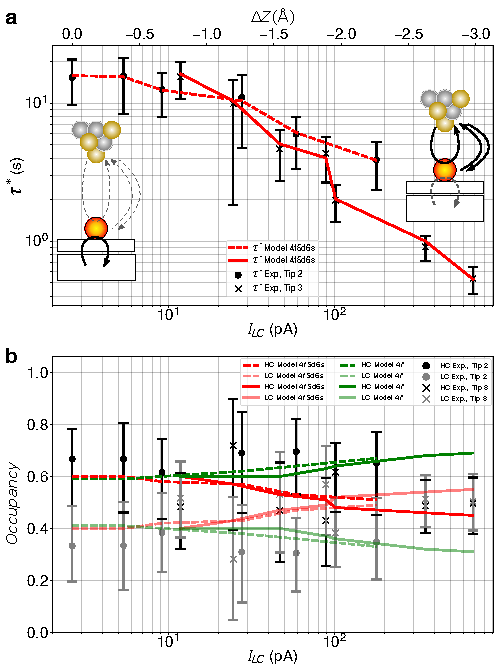
\includegraphics[width=0.5\textwidth]{fig5_final_v3.pdf}
\caption{Variable Current Measurements. (\textbf{a}) Lifetime measurements as a function of average low conductance current and corresponding $\Delta Z$ (\AA) distance ($V_{b} = +1$ mV, $T = 6.5$ K). Two datasets are included, indicated with \circle (Tip 1) or $\times$ (Tip 2), to cover the widest possible current range. $\Delta Z = 0$ is fixed by the lowest current point. (\textbf{b}) Occupancy measurements for each point in (\textbf{a}). Error bars correspond to 95$\%$ confidence intervals calculated using the Agresti-Coull method for binomial distributions \citep{agresti1998}. 
\label{fig:current} }
\end{figure}

Fig.~\ref{fig:current} shows the occupancy and lifetimes as a function of low conductance current $I_{LC}$, taken at $V_{b} = +1$ mV. In the low current regime, substrate-substrate electron scattering $e^{-}_{SS}$ and the tip field $B_{tip}$ are the dominant mechanisms that determine state occupancy and lifetime. The tip field is aligned with the majority spin state at the Fermi level, evidenced by the preferred high conductance state (Fig.~\ref{fig:current}b). As the current is increased, and the tip is moved closer to the Dy adatom, tip-substrate $e^{-}_{TS}$ and tip-tip electron scattering $e^{-}_{TT}$ play a larger role and compete with the aforementioned mechanisms. At positive bias, corresponding to tip-to-substrate tunneling, spin processes parallel to the tip majority spin state at the Fermi level are dominant. If $\rho_{T \uparrow} > 0.5$, this corresponds to spin-increasing, while $\rho_{T \downarrow} > 0.5$ corresponds to spin-decreasing. For $\rho_{T \uparrow} > 0.5 $, the high conductance state corresponds to positive $\ket{m_{+i}}$ states, and the dominant spin-increasing transitions force the adatom out of the $\ket{m_{7}}$ state into the $\ket{m_{8}}$ excited state. In the \textit{4f5d6s} model, QTM from the $\ket{m_{8}}$ state to the $\ket{m_{-8}}$ state results in magnetization reversal. Next, the polarized tunneling electrons promote a rapid de-excitation to the $\ket{m_{-7}}$ state. Promotion to the higher energy $\ket{m_{-5}}$ state is less likely, and the adatom is pinned in the $\ket{m_{-7}}$ state, resulting in a preferred low conductance state. Thus, as tip-substrate $e^{-}_{TS}$ scattering increases, the occupancy of the low conductance state increases. The experimental points in Fig.~\ref{fig:current}b follow this trend. 

This trend in occupancy is able to be reproduced only by the \textit{4f5d6s} model. The \textit{4f} model is characterized by a single reversal pathway through $\ket{\pm 6}$. For $\rho_{T \uparrow} > 0.5 $, the spin-increasing processes that dominate imply that reversal through this pathway from the $\ket{7}$ state is less likely than excitations to the $\ket{8}$ state. Once in the $\ket{8}$ state, the adatom is pinned in the high conductance alignment. For the few reversals that do occur via the pathway $\ket{7}$ \xrightarrow{} $\ket{6}$ \xrightarrow{} $\ket{-6}$ \xrightarrow{} $\ket{-7}$, rapid reversal back to the high conductance state dominates due to the spin-increasing processes. As a result, the \textit{4f} model exhibits an increasing asymmetry towards the high conductance state as tip-substrate $e^{-}_{TS}$ scattering increases. This trend is not compatible with the experimental measurements. 

Note that in either model case, if the tip polarization is reversed (\textit{i.e.} $\rho_{T \downarrow} > 0.5$), the high conductance state corresponds instead to the $\ket{m_{-i}}$ states, spin-decreasing processes are dominant at positive bias, and the aforementioned reversal processes remain valid. The sign of the $\ket{m_{\pm i}}$ states is simply reversed. There is no distinguishable difference between the \textit{4f} model and \textit{4f5d6s} model lifetimes, therefore only the \textit{4f5d6s} model is shown in Fig.~\ref{fig:current}a. In order to fit these experimental characteristic lifetimes, a decreasing $B_{tip}$ is needed for both models (see Supplementary). While the free parameters used to fit the experimental data allow some flexibility, it is not possible to find a set of parameters within the \textit{4f} model that reproduce the slope of the Arrhenius plot and in the high current regime of the variable current occupancy. This is due to the fundamental difference between the \textit{4f} and \textit{4f5d6s} models: the level schemes and the reversal pathways allowed within each scheme. This emphasizes the importance of including the polarized \textit{5d6s} shell to model the spin dynamics of the Dy system.

\begin{figure*}[ht!]
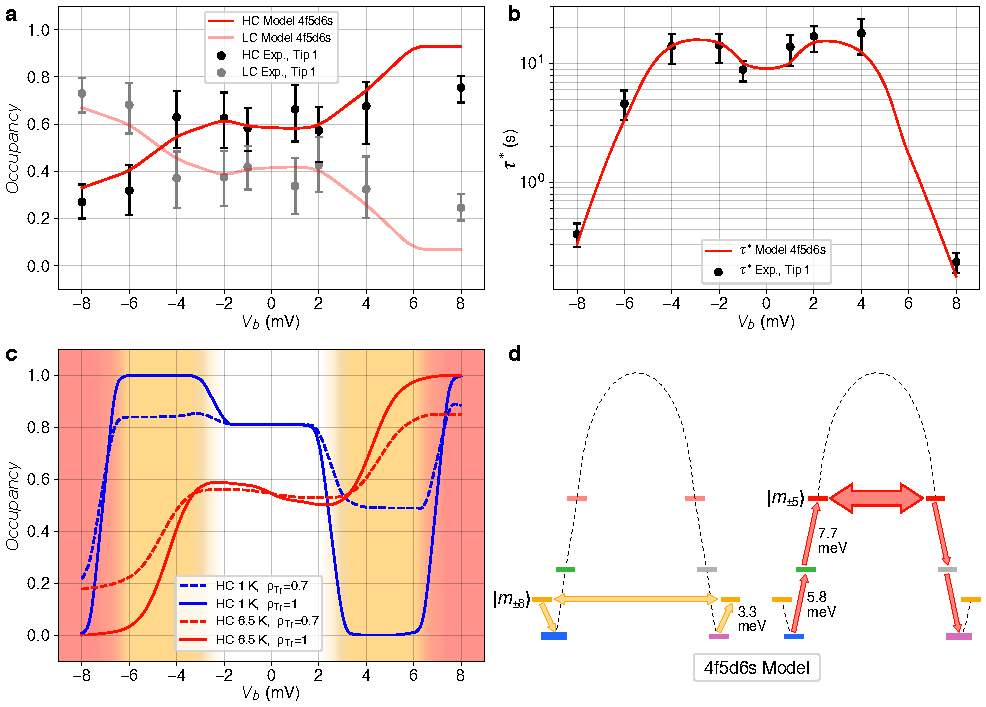
\includegraphics[width=0.99\textwidth]{Fig4_new.pdf}
\caption{Variable Bias Measurements. (\textbf{a}) Experimental lifetime measurements (black) and model prediction (red) as a function of bias ($T = 6.5$ K, see Supplementary for $I$ values). (\textbf{b}) Corresponding occupancy measurements for each point in (\textbf{a}) with the model prediction. The average measured ratio $I_{MR}/I_{o}$ = 0.18±0.05 while the model predicted value is $I_{MR}/I_{o}$ = 0.11. (\textbf{c}) Model predictions of state occupancy as a function of bias at 1 K (blue) and 6.5K (red) for $\rho_{T \uparrow}$ = 1 (solid) and 0.7 (dashed). Note that for simplicity, the tip field $B_{tip}$ (100 mT) and $I_o$ (15 pA) is kept constant for each bias, unlike in (\textbf{a}) and (\textbf{b}). (\textbf{d}) Level scheme and the dominant reversal pathway for each regime in (\textbf{c}). Error bars in (\textbf{a}) and (\textbf{b}) correspond to 95$\%$ confidence intervals calculated using the Agresti-Coull method for binomial distributions \citep{agresti1998}.   
\label{fig:bias} }
\end{figure*}

Fig.~\ref{fig:bias}a and b show the occupancy and lifetimes measured as a function of bias and the corresponding polarized model prediction at $T=6.5$ K. One can clearly see a spin-torque effect at bias voltages $V_d=+8 $ mV and $V_d=-8 $ mV. At  positive biases, corresponding to tip-to-substrate tunneling, the high conductance state is preferred, while at negative biases, corresponding to substrate-to-tip tunneling, the low conductance state is preferred \cite{Khajetoorians2013,delgadoSpinTransferTorqueSingle2010,balashovInelasticElectronmagnonInteraction2008,krause_joule_2011}. The processes that determine the trends in occupancy can be characterized into three regimes. To better elucidate these regimes, and put the variable temperature and current trends into a better context, Fig.~\ref{fig:bias}c displays the \textit{4f5d6s} model prediction at $T=1$ K for a fully polarized tip $\rho_{T \uparrow} = 1 $ (blue solid line). For biases between $\pm 2$ meV (white background in Fig.~\ref{fig:bias}c), the occupancy is determined by the tip field $B_{tip}$ which shifts the $\ket{m_{7}}$ state to the lowest energy. Substrate electrons excite the adatom towards the $\ket{m_{\pm8}}$ states in which QTM enables the reversal of the magnetization.

At biases between $+3$ and $+7$ meV (yellow shaded area in Fig.~\ref{fig:bias}c), tunneling electrons can promote transitions towards the first excited states $\ket{m_{\pm 8}}$. For $\rho_{T \uparrow} > 0.5 $, the high conductance state corresponds to positive $\ket{m_{+i}}$ states, and tip-to-substrate tunneling is dominated by spin-increasing transitions. The left sketch in Fig.~\ref{fig:bias}d illustrates the reversal pathway allowed at these energies. Only spin increasing transitions are possible due to the complete tip polarization $\rho_{T \uparrow} = 1$. This forces the adatom out of the $\ket{m_{7}}$ state into the $\ket{m_{8}}$ excited state, in which a QTM process induces the crossing of the MAE barrier towards the $\ket{m_{-8}}$ state. Next, the polarized tunneling electrons promote a rapid de-excitation in the $\ket{m_{-7}}$ state. It is clear that this process pins the adatom in the $\ket{m_{-7}}$ state, corresponding to the low conductance state for a tip polarization $\rho_{T \uparrow} > 0.5 $. 

At biases above $+7$ meV (red shaded area in Fig.~\ref{fig:bias}c), transitions between the ground states $\ket{m_{\pm7}}$ and higher excited states $\ket{m_{\pm 6, \pm 5}}$ occur, enabling the magnetization reversal through QTM via $\ket{m_{\pm 5}}$. For $\rho_{T \uparrow} = 1 $, tip-to-substrate tunneling is still completely dominated by spin-increasing transitions, but now the reversal pathway (right sketch in Fig.~\ref{fig:bias}d) forces the Dy adatom into the $\ket{m_{7}}$ state, corresponding to the high conductance state. This process (Fig.~\ref{fig:bias}d, right) dominates over the previous one (Fig.~\ref{fig:bias}d, left) because the QTM channel between $\ket{m_{\pm 5}}$ is $>10^3$ times more efficient than between $\ket{m_{\pm 8}}$. 

The situation is reversed at negative biases, as shown in Fig.~\ref{fig:bias}c: substrate-to-tip tunneling is dominated by spin-decreasing transitions, which force the HC state for $-7<V_d<-3$ meV and LC state for $V_d<-7$ meV. Notice that flipping the polarization of the tip would reverse the occupancy only between $-3<V_d<3$ meV, in which the asymmetry is dominated by the tip field and not by the polarization of tunneling electrons. Partially polarized currents (\textit{e.g.} dashed lines in Fig.~\ref{fig:bias}c) results in a softened spin-torque effect that cannot completely overcome the effect of the tip field, as one can see in the blue dashed curve for $3<V_d<7$ meV in Fig.~\ref{fig:bias}c.  Fig.~\ref{fig:bias}c shows how the temperature smears the regimes: the step in the occupancy at high bias ($|V_d|>7$ meV) overcomes the effect of the spin-torque at intermediate bias ($2<|V_d|<7$ meV), which in turn compensates the asymmetry induced by the tip field at low bias ($|V_d|<3$ meV). Thus, the variable temperature measurements presented in Fig.~\ref{fig:temp} explore the effect of increasing this smearing, resulting in an increase in magnetization reversals through the $\ket{m_{\pm 5}}$ states at higher temperatures. On the other hand, the variable current measurements in Fig.~\ref{fig:current} explore the effect of increasing tip-generated scattering processes relative to substrate scattering processes; stressing the importance of the reversal pathways available at low bias and at $T=6.5$ K. Note that as a result of this temperature smearing, we find no appreciable difference between the \textit{4f} and \textit{4f5d6s} model in fitting the experimental trends as a function of bias (see Supplementary).



\bibliographystyle{naturemag}
\bibliography{bib.bib}

\end{document}

